\section{Theorie}
\label{sec:Theorie}
\subsection{Ablenkung von Elektronen im elektrischen Feld}
\label{sec:efeld}
Bewegen sich Elektronen mit einer konstanten Geschwindigkeit $v_z$ durch ein orthogonal zur Bewegungsrichtung verlaufendes homogenes elektrisches Feld, so werden
sie durch die Coulomb-Kraft abgelenkt. Wird das homogene Feld durch einen Kondensator mit der Spannung $U_d$, dem Plattenabstand $d$ und der Länge
$p$ erzeugt, ergibt sich für die Geschwindigkeit in die Ablenkungsrichtung $y$ der Elektronen folgender Ausdruck:
\begin{equation}
  v_y = \frac{e_0}{m_0} \frac{U_d}{d} \frac{p}{v_z}
  \label{eqn:vy}
\end{equation}
mit der Elektronenmasse $m_0$ und der Elementarladung $e_0$.
Da sich die Elektronen in einer Kathodenstrahlröhre, welche in \ref{sec:Durchführung} beschrieben wird, befinden, wird nun die Ablenkung der Elektronen von
dem Fall $U_d = 0$, welche auf dem Leuchtschirm der Kathodenstrahlröhre sichtbar ist, berechnet.
Der schematische Aufbau für welchen die Ablenkung berechnet werden soll ist in Abbildung \ref{fig:efeld} zu sehen.
\begin{figure}
  \centering
  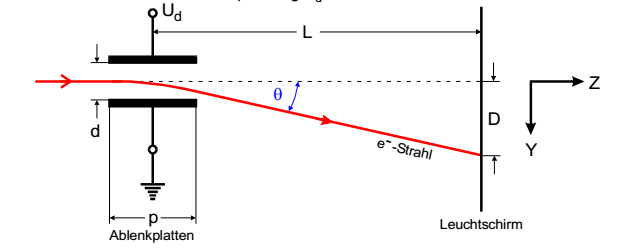
\includegraphics{images/efeld.png}
  \caption{Schematischer Aufbau der Ablenkung im elektrischen Feld \cite{501}.}
  \label{fig:efeld}
\end{figure}
Aus dem Winkel $\Theta = \sfrac{v_y}{v_z}$, der Gleichung \eqref{eqn:vy} und der durch die Kathodenstrahlröhre vorgegebenen Geschwindigkeit $v_z = e_0 U_B$ lässt sich
für die Ablenkung $D$ folgende Gleichung herleiten:
\begin{equation}
  D = \Theta \, L =  \frac{p}{2d} L \frac{U_d}{U_B}.
  \label{eqn:Ablenkung}
\end{equation}
Dabei ist $L$ die Länge, welche der Elektronenstrahl nach der Ablenkung bis zum Leuchtschirm noch zurücklegen muss.

\subsection{Ablenkung von Elektronen im magnetischen Feld}
\label{sec:bfeld}
